
\begin{figure}[b]
    \centering
    \vspace{-0.5cm}
    \begin{subfigure}[b]{0.49\textwidth}
        \begin{subfigure}[b]{0.4\textwidth}
            \center
            Context $s_0$ \vspace{0.2cm}
        \end{subfigure}
        \begin{subfigure}[b]{0.59\textwidth}
            \adjustbox{trim=0 0 {0.5\width} 0,clip} {
                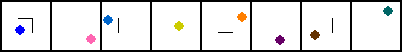
\includegraphics[width=1.7\linewidth]{ccrig/img/cvae_samples/wall_pointmass1_x0.png}
            }
        \end{subfigure}

        \vspace{0.1cm}

        \begin{subfigure}[b]{0.4\textwidth}
            \center
            CVAE samples \vspace{1cm}
        \end{subfigure}
        \begin{subfigure}[b]{0.59\textwidth}
            \adjustbox{trim=0 0 {0.5\width} 0,clip} {
                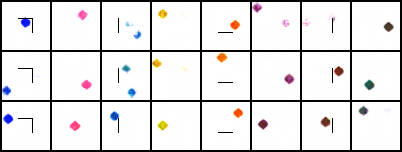
\includegraphics[width=1.7\linewidth]{ccrig/img/cvae_samples/wall_pointmass1_cvae_samples.png}
            }
        \end{subfigure}

        \vspace{0.1cm}

        \begin{subfigure}[b]{0.4\textwidth}
            \center
            VAE samples \vspace{1cm}
        \end{subfigure}
        \begin{subfigure}[b]{0.59\textwidth}
            \adjustbox{trim=0 0 {0.5\width} 0,clip} {
                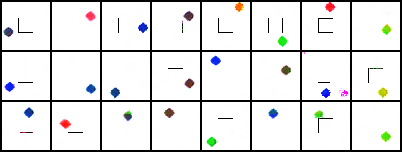
\includegraphics[width=1.7\linewidth]{ccrig/img/cvae_samples/wall_pointmass1_vae_samples.png}
            }
        \end{subfigure}
    \end{subfigure}
    \hfill
    \begin{subfigure}[b]{0.49\textwidth}
        \begin{center}
            Multi-color 2D Navigation Training Rollouts \vspace{0.1cm}
        \end{center}

        \hspace{0.2cm} $s_0$ \hspace{3.7cm} $s_H$ \hspace{0.7cm} $d(\bar{z}_g)$

        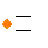
\includegraphics[width=0.14\linewidth]{ccrig/img/pointmass_vae_rollout/0/0.png}
        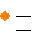
\includegraphics[width=0.14\linewidth]{ccrig/img/pointmass_vae_rollout/0/1.png}
        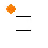
\includegraphics[width=0.14\linewidth]{ccrig/img/pointmass_vae_rollout/0/2.png}
        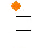
\includegraphics[width=0.14\linewidth]{ccrig/img/pointmass_vae_rollout/0/3.png}
        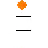
\includegraphics[width=0.14\linewidth]{ccrig/img/pointmass_vae_rollout/0/4.png}
        \hspace{0.3cm}
        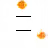
\includegraphics[width=0.14\linewidth]{ccrig/img/pointmass_vae_rollout/0/goal.png}

        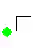
\includegraphics[width=0.14\linewidth]{ccrig/img/pointmass_vae_rollout/1/0.png}
        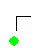
\includegraphics[width=0.14\linewidth]{ccrig/img/pointmass_vae_rollout/1/1.png}
        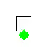
\includegraphics[width=0.14\linewidth]{ccrig/img/pointmass_vae_rollout/1/2.png}
        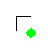
\includegraphics[width=0.14\linewidth]{ccrig/img/pointmass_vae_rollout/1/3.png}
        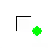
\includegraphics[width=0.14\linewidth]{ccrig/img/pointmass_vae_rollout/1/4.png}
        \hspace{0.3cm}
        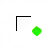
\includegraphics[width=0.14\linewidth]{ccrig/img/pointmass_vae_rollout/1/goal.png}

        \begin{center}
            Multi-color 2D Navigation Test Rollouts \vspace{0.1cm}
        \end{center}

        \hspace{0.2cm} $s_0$ \hspace{3.7cm} $s_H$ \hspace{0.8cm} $s_g$

        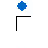
\includegraphics[width=0.14\linewidth]{ccrig/img/pointmass_env_rollout/0/0.png}
        
\includegraphics[width=0.14\linewidth]{ccrig/img/pointmass_env_rollout/0/1.png}
        
\includegraphics[width=0.14\linewidth]{ccrig/img/pointmass_env_rollout/0/2.png}
        
\includegraphics[width=0.14\linewidth]{ccrig/img/pointmass_env_rollout/0/3.png}
        
\includegraphics[width=0.14\linewidth]{ccrig/img/pointmass_env_rollout/0/4.png}
        \hspace{0.3cm}
        
\includegraphics[width=0.14\linewidth]{ccrig/img/pointmass_env_rollout/0/goal.png}

        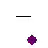
\includegraphics[width=0.14\linewidth]{ccrig/img/pointmass_env_rollout/1/0.png}
        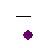
\includegraphics[width=0.14\linewidth]{ccrig/img/pointmass_env_rollout/1/1.png}
        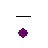
\includegraphics[width=0.14\linewidth]{ccrig/img/pointmass_env_rollout/1/2.png}
        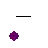
\includegraphics[width=0.14\linewidth]{ccrig/img/pointmass_env_rollout/1/3.png}
        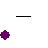
\includegraphics[width=0.14\linewidth]{ccrig/img/pointmass_env_rollout/1/4.png}
        \hspace{0.3cm}
        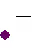
\includegraphics[width=0.14\linewidth]{ccrig/img/pointmass_env_rollout/1/goal.png}
    \end{subfigure}

    \caption{The pointmass environment is shown. Left, we compare samples from our CC-VAE model to a standard VAE. The initial image $s_0$ is shown on the top row, and samples conditioned on $s_0$ are shown below. Our model coherently maintains object color and geometry in its samples, suggesting that the context conditioned model can successfully factor out the scene-specific object identity from the variable object position. This enables the use of the CC-VAE for goal proposals in visually diverse scenes. Right, rollouts from CC-RIG are shown. We see that during collecting training rollouts, the policy succeeds in coherent exploration by generating reachable goals. Then, given a goal image at test time, the policy successfully reaches the goal. 
    Videos of rollouts on all environments, both simulation and real-world, can be found at  \url{https://ccrig.github.io/}
    }
    \label{fig:pointmass}
\end{figure}

\section{Multi-Color 2D Navigation Experiments} \label{sec:pointmass}

In order to study generalizing to varying appearance and dynamics with CC-RIG, we introduced the multi-color 2D point navigation environment shown in \ref{fig:pointmass}. The goal is to navigate a point robot around the central walls. The arrangement of the walls is randomly chosen from a set of 15 possible configurations in each rollout, and the color of the circle indicating the position of the point robot is generated from a random RGB value. Thus at test time, the agent sees new colors it has never trained on.

First, we see from the samples in~Figure~\ref{fig:pointmass} that the learned latent space for the CC-VAE is more reasonable than a VAE: it preserves color and wall information in samples and represents only the colored circle position in the latent variable $z_t$. This improves the capability of our algorithm to learn in several ways: it provides a more informative reward function, and gives us better goal sampling for both exploration rollouts and experience relabeling when training the Q function.

Learning curves obtained by training the different methods above in this environment are presented in the main paper Figure~\ref{fig:sim-learning-curves}. This task is trivial for the oracle method to learn, as it directly receives state information and does not need to generalize between different object appearances. CC-RIG requires more samples to learn, but eventually approaches the oracle performance. RIG plateaus with poor performance in comparison.

\pagebreak

\section{Off-Policy Experiments}

Because we use off-policy RL methods, one major benefit is that we can bootstrap training from large interaction datasets rather than requiring on on-policy data collection. This is particularly vital in the real-world, where on-policy data collection is expensive in terms of human effort, and repeatedly tuning on-policy methods for complex tasks is likely to be impractical. Our robot experiments are therefore run by starting with a fixed initial dataset of 50,000 samples (about 3 hours) of random interaction with 20 objects, which is used for both training the CC-VAE as well as RL. Our simulated experiments are conducted with online data-collection to make comparison with prior work clearer, but in this section we show that bootstrapping with off-policy training is possible in these settings as well.

In our simulated experiments, we first collect 100,000 samples (1000 trajectories) with random actions. This data is used both to train the CC-VAE and as off-policy data. When we begin RL, we load these samples into the replay buffer and perform 100,000 gradient updates of RL. As shown in Figure \ref{fig:offpolicy}, this allows us to begin online data collection with a reasonably good policy. But we see that online data collection does improve slightly beyond this initial policy. In dynamically sensitive environments or environments where random actions do not provide meaningful interaction, this online data collection may still be very valuable.

\begin{figure}[t]
    \centering
    \begin{subfigure}[b]{0.48\textwidth}
        \center
        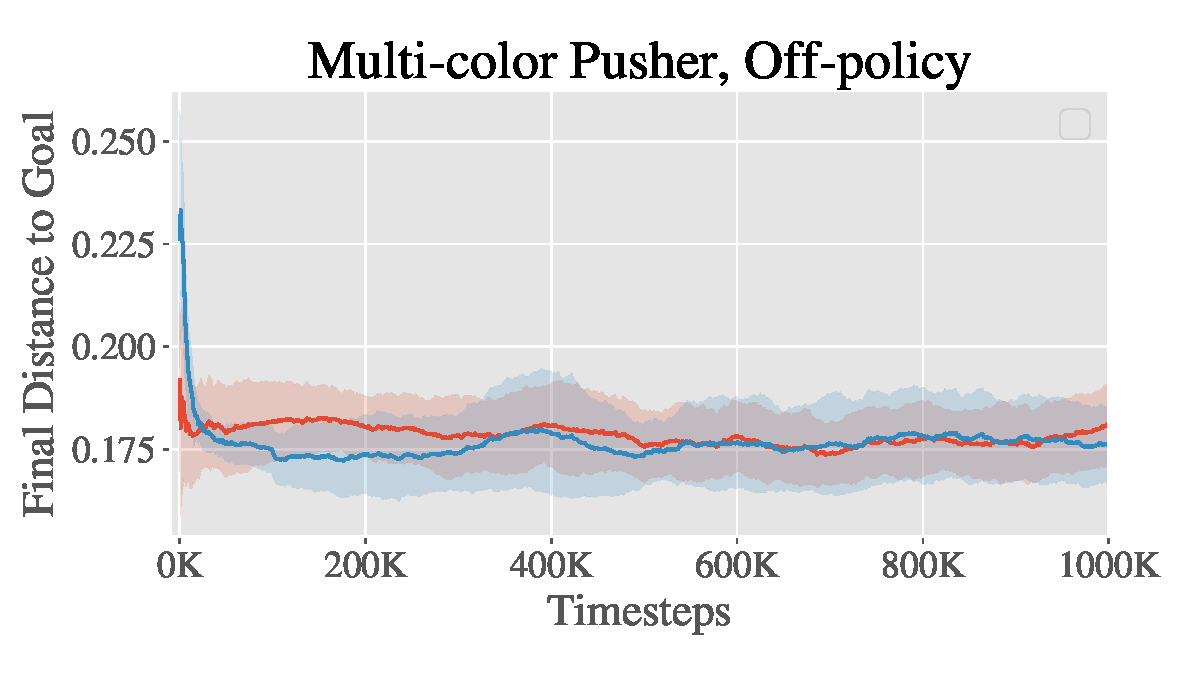
\includegraphics[height=3.8cm]{ccrig/img/offpolicy_pusher_camera_ready-crop.pdf}
    \end{subfigure}
    \hspace{0.3cm}
    \begin{subfigure}[b]{0.48\textwidth}
        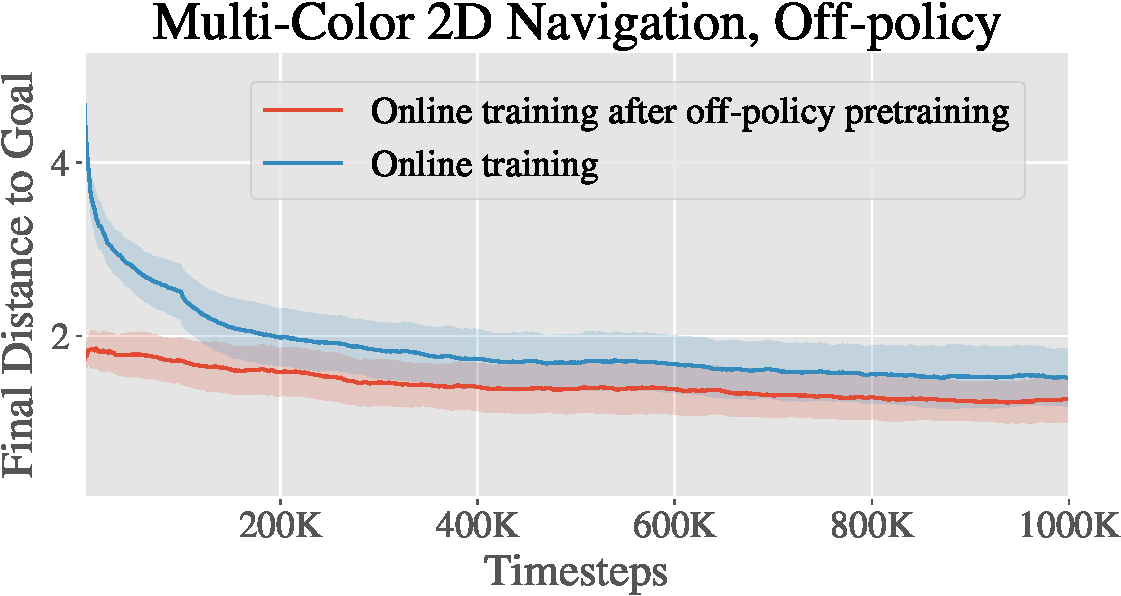
\includegraphics[height=3.8cm]{ccrig/img/offpolicy_pointmass_camera_ready-crop.pdf}
    \end{subfigure}
    \caption{Off-policy learning results in simulated environments. These experiments begin with 100K samples from random interaction loaded into the replay buffer. The red lines (off-policy pre-training) additionally do 100K steps of Q learning before starting on-line data collection. We see that off-policy pre-training results in proficient initial performance from a fixed dataset, which is extremely useful in domains such as robotics where collecting new samples is expensive.}
    % \vspace{-0.2in}
    \label{fig:offpolicy}
\end{figure}
